\chapter{ランサムウェア対策}
\section{感染リスクの緩和}
現実世界の攻撃を戦術と使用技術の観点から分類したフレームワークであるMITRE ATT\&CK \cite{MITREATT12:online}によると,
ランサムウェアのデータ侵害は,攻撃の最終段階であるImpactステージの
Data Destruction,
Data Encrypted for Impact,
Data Manipulation
のいずれかに分類される.
つまり,ランサムウェアによるデータ侵害はInitial Access (初期アクセス) や Privilege Escalation (権限昇格) などのステージを完了した後に発生するといえる.
したがって,Impactより前のステージにおけるセキュリティ強化もランサムウェア対策の重要な要素である.
なお,本研究の提案手法はランサムウェアのImpactステージの活動に対する対策であるため,本節の内容はスコープ外であることに注意する.
\begin{figure}[t]
  \begin{center}
    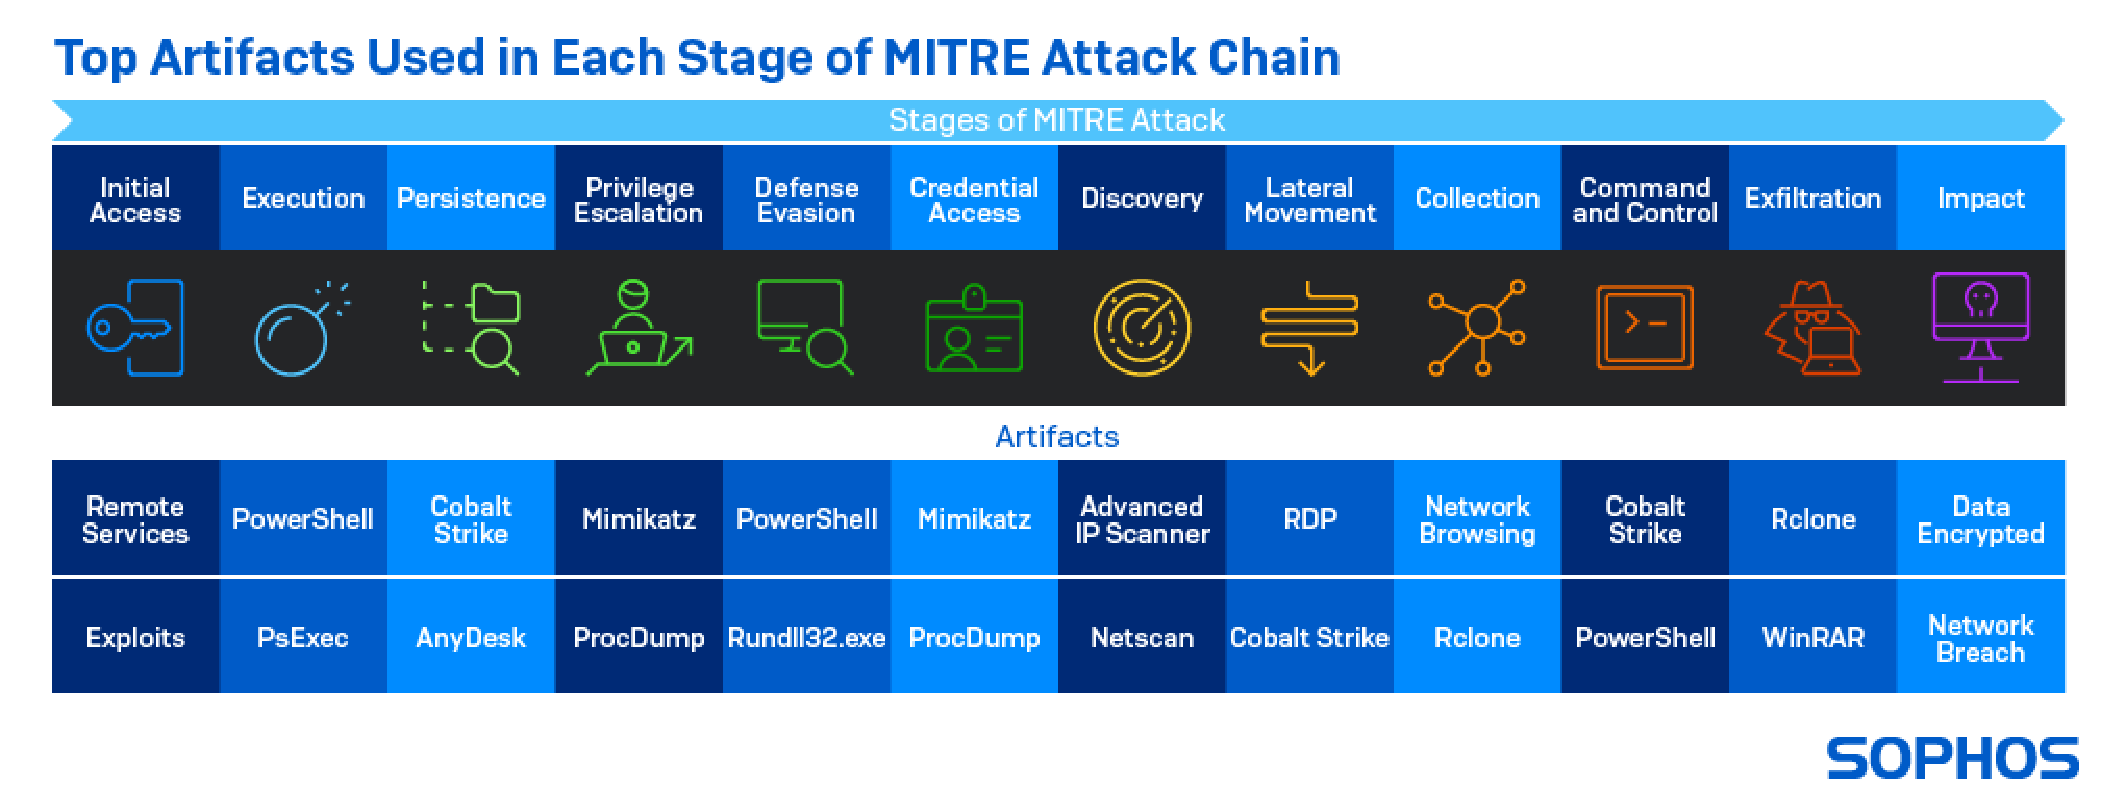
\includegraphics[width=0.8\columnwidth]{doc/img/mitre-attack-chain.eps}
  \end{center}
  \caption{Overview of each stage in MITRE ATT\&CK framework.
    Some stages such as Reconnaissance are omitted for simplicity. \cite{mitre-explained}}
  \label{fig:mitre-attack-chain}
\end{figure}

本節では,すべてのランサムウェアが通過するステージであるInitial Accessステージに焦点を当て,感染リスクの緩和について述べる.
SpyCloud社 \cite{spycloud-ransomware} によると,ランサムウェアのInitial Accessに利用される手法として2023年に最も多く報告されたものは
フィッシング,サードパーティアプリケーションのIAM設定の不備,cookie窃取によるセッションハイジャックであった.
これらの手法に対する一般的な対策を\tabref{tab:initial-access}に示す.
\begin{table}[t]
  \centering
  \label{tab:initial-access}
  \caption{Techniques for Initial Access and general countermeasures}
  \begin{tabular}{|c|c|}
    \hline
    \textbf{Initial Accessの手法} & \textbf{対策} \\
    \hline
    フィッシング                     &
    \begin{tabular}{c}
      メールフィルタリングを強化する \\
      組織構成員の教育を行う
    \end{tabular}
    \\
    % Email filteringUser awareness training,         \\
    \hline
    IAM設定の不備                   &
    \begin{tabular}{c}
      多要素認証を導入する
      % Email filtering \\ User awareness training
    \end{tabular}
    \\
    \hline
    Cookie窃取によるセッションハイジャック     &
    \begin{tabular}{c}
      Secure属性やHTTPOnly属性を強制する \\
      多要素認証を導入する
    \end{tabular}
    \\
    \hline
  \end{tabular}
\end{table}

\section{ランサムウェア検知}
\subsection{特徴量}
ランサムウェアを検知する手法で用いられる特徴量は,
実行ファイルの解析から得られる静的データと,実行ファイルを実行した際にプロセスの振る舞いから得られる動的データに分類される.
静的データを用いた検知を静的検知,動的データを用いた検知を動的検知と呼ぶ.
静的検知と動的検知は組み合わせて使用されることもあり,これをハイブリッド検知と呼ぶ.

静的検知では実行ファイルにおけるランサムウェア特有の構造的特徴を分析する.
典型的な静的データはファイルのハッシュ値,文字列,関数呼び出しなどである .
文字列としては"ransom"や"bitcoin"などのランサムノートに頻出する文字列や,
過去にランサムウェアが使用していたドメイン文字列やIPアドレスなどが確認される\cite{berrueta2019survey}.
また関数呼び出しについては,暗号化やファイルアクセスといった操作の有無を,ランサムウェアと良性アプリケーションの区別に使用することができる \cite{Evolution-Ransomware}.
しかし,静的データは一般に難読化や圧縮などの手法に弱く,さらに新種のランサムウェアに対して有効ではないことが多いという問題が指摘されている \cite{mitigation-modern}.

動的検知では実行中のプロセスの振る舞いを分析する.
ランサムウェアは特定のディレクトリ以下のファイル一覧を取得して各ファイルを暗号化する挙動を繰り返し行うことから,
ファイルシステム上の操作,暗号化ライブラリやAPIの呼び出しが特徴量として使用されることが多い \cite{Evolution-Ransomware}.
またランサムウェアがファイルに書き込むデータは暗号化されているため,
書き込まれるデータのエントロピーを利用する手法も複数存在する \cite{kharaz2016unveil,kharraz2017redemption}.
ただし書き込みデータのエントロピーはファイル圧縮などの正常アプリケーションにおいても高くなるので,エントロピーはその他の特徴量と組み合わせて使われる傾向がある \cite{berrueta2019survey}.

\subsection{検知レイテンシ}
動的検知あるいはハイブリッド検知において,ランサムウェアが実行されてから検知されるまでの時間を本稿では検知レイテンシと呼ぶ.
検知レイテンシが小さければランサムウェアの被害を抑えることができるため,検知手法の評価指標として重要である.
例えばRATAFIA \cite{alam2019ratafia} はオートエンコーダを用いた検知手法で,WannaCryを含む変種を最大5.3秒で検知した.
また,RWGuard \cite{mehnaz2018rwguard} はデコイファイル,プロセス監視,ファイル監視を組み合わせてレイテンシの削減を目指した手法であり,
評価実験ではランサムウェアのプロセスを9秒未満で特定した.
Brownorら \cite{brownor2024ransomware} は提案した検知手法の検知レイテンシをCPU使用率ごとに測定し,
使用率が90\%の設定でも評価に用いたランサムウェアサンプルを3秒未満で検知することができた.

検知レイテンシはランサムウェア攻撃を迅速に終了させられるかどうかという観点において重要な指標であるが,
検知レイテンシの評価を行っている研究が少ないことが指摘されている\cite{alam2019ratafia}.
例えばいくつかの研究では,提案手法の検知精度を最大化するために,30日間などの非常に長い期間での評価を行っているものがある \cite{mitigation-modern}.

\section{ランサムウェア被害からの復旧}
ランサムウェア被害からの復旧とは,ランサムウェアによって侵害されたデータを\textbf{身代金を支払うことなく}攻撃前の状態に戻すことを指す.
したがって復旧手法は,データの復旧を実施するトリガとして,人間の明示的な入力または手法自体の自動的なランサムウェア検知を必要とする.

\subsection{スナップショットによる復旧}
スナップショットとは,特定の時点でのファイルシステムやデータの状態を記録する機能である.
ランサムウェア攻撃が発生する前に取得したスナップショットを用いることで,攻撃前の状態にデータを復元することができる.
そのため一定間隔でスナップショットを取得し,隔離されたストレージに保存しておくことはランサムウェア対策として広く採用されている \cite{wang2024ransom}.

ZFS \cite{openzfsz73:online} やBtrfs \cite{BTRFS—Th72:online}はファイルシステムとしてネイティブにスナップショット機能を提供している.
ZFSは差分スナップショット方式を採用しており,スナップショット取得後に更新されたファイルのみをCOW (Copy-On-Write) によってコピーする.
これによりスナップショット作成を高速に行い,ストレージ容量を節約している.
ZFSのスナップショットはファイルシステム単位で作成され,スナップショットを取得したファイルシステム上に保存される.
BtrFSもZFSと同様に差分スナップショット方式をサポートするが,スナップショットはサブボリューム単位で作成される.
サブボリュームはファイルシステム上でディレクトリとして扱えるデータ領域で,ユーザが作成・削除することができるため
ZFSよりも柔軟なスナップショット管理が可能である.



\subsection{暗号化鍵の取得による復旧}
\ref{subsec:encrypt-algo}節で述べたように,共通鍵暗号では暗号化と復号に同じ鍵を使用する.
そのため共通鍵暗号を利用するランサムウェアに対しては,暗号化に使用される鍵を取得することができればデータを復号することができる.
PayBreak \cite{kolodenker2017paybreak} はこの点に着目して開発された手法で,Windows OSが提供する暗号化ライブラリを
フックして暗号化鍵を取得する.
取得された鍵は事前にユーザが登録した公開鍵によって暗号化されたのち,追記のみが可能なデータストアに保存される.
\begin{figure}[t]
  \begin{center}
    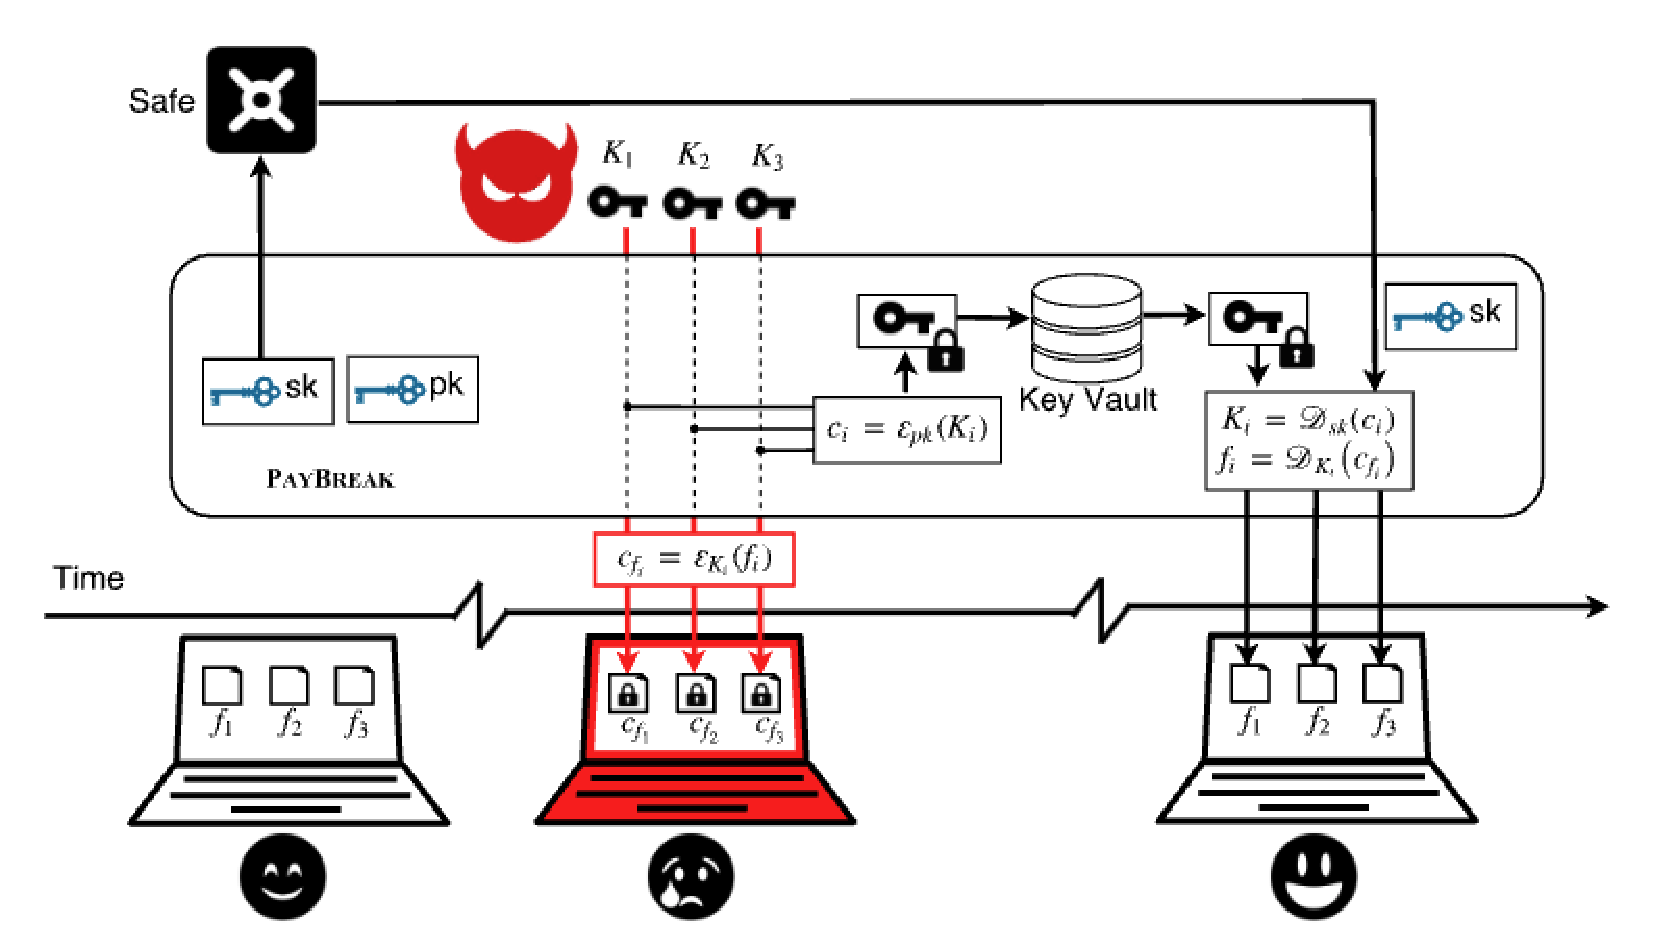
\includegraphics[width=0.8\columnwidth]{doc/img/paybreak-overview.eps}
  \end{center}
  \caption{Overview of PayBreak. \cite{kolodenker2017paybreak}}
  \label{fig:paybreak-overview}
\end{figure}
PayBreakは暗号化ライブラリの動的リンクと静的リンクの両方に対応している.
さらに代替となる暗号化ライブラリが登場した場合でも,マルウェア解析によって一度暗号化関数を特定することができれば,
その関数をフック対象として容易に追加することができる.
しかしながら,PayBreakは非対称鍵暗号を利用するランサムウェアには対応していない.

\subsection{SSDの特性を利用した復旧}
SSDの特性を活用してランサムウェアにより侵害されたデータを復旧する手法が提案されている.
HDDとSSDはブロックデバイスとしての抽象化により論理的には同一のI/O操作を受け付けるが,
ハードウェアレベルではデータ上書き時の挙動が異なる.
HDDでは論理的な上書きに対して物理的な上書きが即時実行される (in-place書き込みされる) 一方で,
SSDにおける物理的な上書きは複数回の論理的な上書きに対してまとめて実行される
(上書きされる古いデータがout-of-place書き込みされ,GC: Garbage Collectionによって一定時間の後削除される).
これはSSD上で物理ページを消去するレイテンシが大きいためである.
つまり,SSDは上書きされたファイルや削除されたファイルのコピーを,GCまでの期間だけ保持することになる.

FlashGuard \cite{huang2017flashguard} は上記のSSDの特性を利用したデータ復旧システムであり,
SSDファームウェアとして実装された.
FlashGuardはランサムウェアによって上書きまたは削除された可能性のある物理ページに「GCによって回収しない」というフラグを立てることで,
SSD上にそのデータを保持してデータ復旧に使用できるようにする.
筆者らは1477個のランサムウェアサンプルを用いてFlashGuardの有効性を評価し,ランサムウェアによって暗号化されたファイルを効率的に復元可能であり
SSDに与える性能劣化も最小限であることを示した.

FlashGuardは保守的にデータの保持を行うため,実際には保持しておく必要がない古いデータまで保持してしまうという問題がある.
SSD-Insider \cite{baek2018ssd} はブロックI/Oリクエストのヘッダを参照してあるデータがランサムウェアによって侵害されたかどうかを判定することで
この問題を改善した.

SSDの特性を活用したこれらの手法は,ランサムウェア検知がデータ復旧のトリガとなるが,
検知において誤検知や見逃しが頻繁に発生する点が先行研究によって指摘されている \cite{han2020effectiveness}.
そのため本来必要のないリカバリが発生してデータが消失するリスクがある \cite{css2024-enomoto}.
さらに,ハードウェアに依存した復旧手法は大規模な展開が難しいという課題も指摘されている \cite{wang2024ransom}.
特殊なハードウェアまたはプロトタイプ的なハードウェアに依存していること,
ランサムウェアの進化に追随してファームウェアを頻繁に更新することが非現実的であるからだ.

\subsection{ファイルシステムの拡張による復旧}
いくつかの先行研究では,ファイルシステムを拡張することでランサムウェアによるデータ侵害からの復旧を実現している.
ShieldFS \cite{shieldFS} はOSのネイティブなファイルシステムにカーネルモジュールを適用し,
任意のプロセスのファイル書き込みまたは削除のI/Oリクエストに対してCOWを行うデータ保護システムである.
概要を\figref{fig:shieldFS}に示す.
ShiledFSはすべてのプロセスの低レベルのI/Oリクエスト,および不審なプロセスの暗号化処理を監視してプロセスごとの悪意スコアを計算するモジュールを持つ.
あるプロセスの悪意スコアが閾値を超えた場合,COWのコピー元となっているファイルを用いて,そのプロセスによって更新されたファイルを復旧する.
Redemption \cite{kharraz2017redemption} はShiledFSと類似した手法で,ファイルシステムへの書き込みおよび削除のI/Oリクエストをインターセプトし,
保護領域に作成されるコピーファイル (「リフレクションファイル」と呼ばれる) にリクエストをリダイレクトする.
リフレクションファイルは変更履歴が保持されており,ランサムウェアによるファイルの暗号化や削除を検知した場合,リフレクションファイルを用いてファイルを復元する.
\begin{figure}[t]
  \begin{center}
    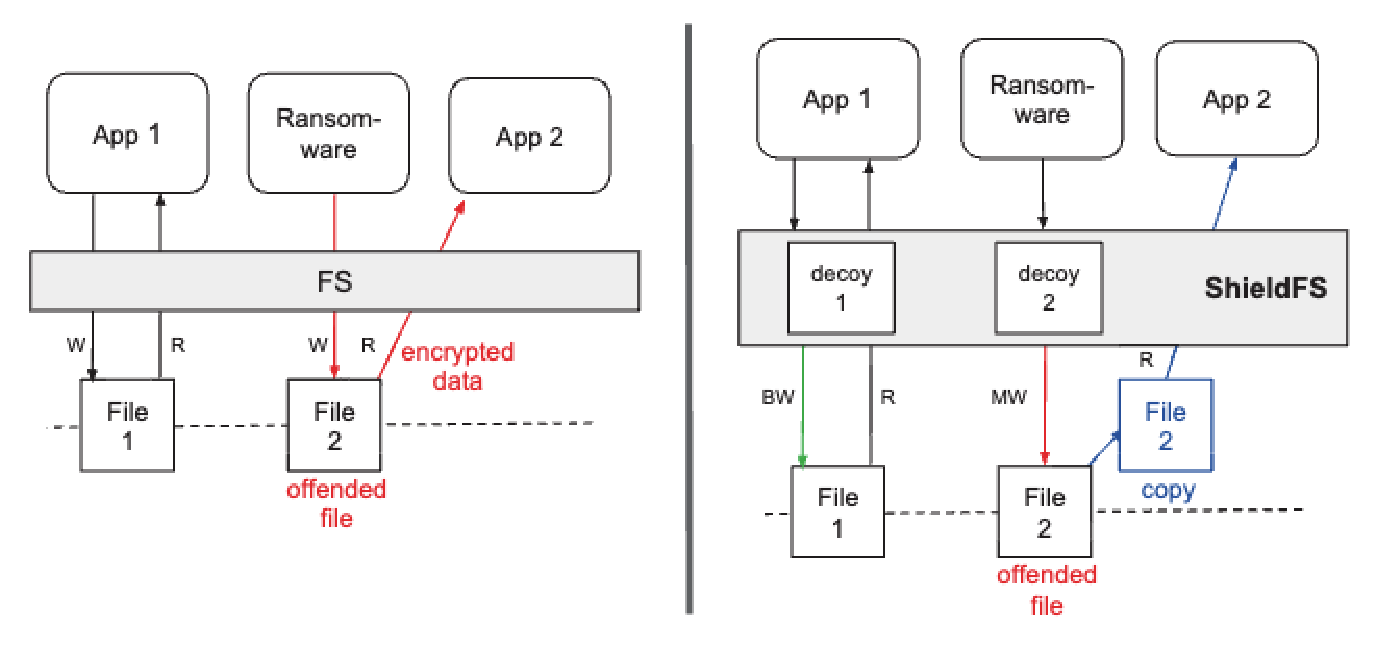
\includegraphics[width=0.8\columnwidth]{doc/img/shieldFS.eps}
  \end{center}
  \caption{On the right ShieldFS shadowing a file offended by ransomware malicious write (MW), in comparison to standard filesystems (on the left). \cite{shieldFS}}
  \label{fig:shieldFS}
\end{figure}

MatosらはRockFS \cite{matos2018rockfs} を提案し,悪意ある第三者によるファイルデータの侵害からの復旧を行うシステムの設計と実装を行なった.
ランサムウェアなどがバックアップサービスのクライアントデバイス上に保存されているデータを侵害すると,データの更新がクラウドに同期されるため,
バックアップが利用不可能になってしまう.
RockFSは既存のクラウドバックアップサービスに存在するこの問題に注目し,
クライアントデバイス上のファイルシステム操作のログをクラウドストレージ上に保存するというアプローチを取っている.
ランサムウェア攻撃が発覚した場合に,ログ上の正常な操作のみをファイルの初期バージョンに適用することでデータを復元する.
攻撃者がクラウドストレージへのアクセス情報を窃取してログを改ざんすることを防ぐために,RockFSはログを完全性を保証するための手法を提案している.
さらにRockFSは操作ログを複数のクラウドストレージに分散して保存する仕組みを提供しており,ログの改ざんを試みる攻撃者は
複数のクラウドサービスに侵入する必要がある点が特徴的である.




